\begin{flushleft}
{\Huge Øhlvisor\\}

\end{flushleft}

\vspace{2cm}
\begin{center}
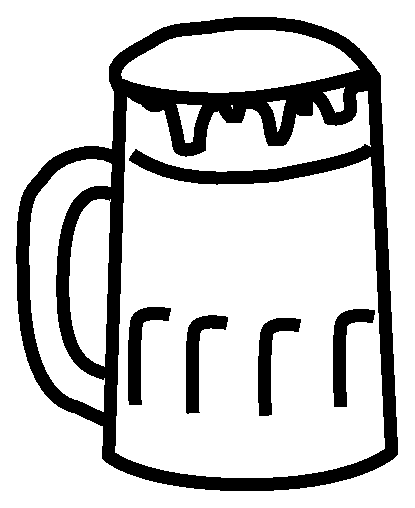
\includegraphics[width=6cm]{bilder/69.eps}

{\Large
\vspace{1cm}
Øhl är gott.
}
\end{center}

\newpage

\begin{song}{Ode till øhlet}{odetillohlet}
\mel{Trampa på gasen}
\begin{vers}
Tu tu tu Tuborg\\
och ca ca ca Carlsberg\\
det är den bästa\\
pi pi pi pilsnern som jag vet\\
\end{vers}
\begin{vers}
Tu tu tu Carlsberg\\
och ca ca ca Tuborg\\
det är det bästa\\
pi pi pi ölet som jag vet\\
\end{vers}
\begin{vers}
Tu tu tu Ölberg\\
och ca ca ca Pilsborg\\
det är den bästa\\
pi pi pi biran som jag vet!\\
\end{vers}
\end{song}

\begin{song}{Lapin Kulta}{lapinkulta}
\mel{Broder Jacob}
\begin{vers}
Lapin kulta, Lapin kulta,\\
Karjala, Karjala\\
Aura sekä Olvi,\\
Aura sekä Olvi,\\
Koff Koff Koff\\
Koff Koff Koff.\\
\end{vers}
\end{song}

\newpage

\begin{song}{Jag var full en gång}{jagvarfullengang}
\mel{Flottarkärlek}
\begin{vers}
Jag var full en gång för längesen\\
på knäna kröp jag hem\\
varje dike var för mig ett vilohem.\\
I varje hörn i varje vrå\\
hade jag en liten vän\\
ifrån Renat upp till nittiosex procent\\
\end{vers}
\begin{vers}
Jag var full en gång för länge sen\\
på knäna kröp jag hem\\
och i sällskap hade jag en elefant.\\
Elefanten spruta vatten\\
och jag trodde det var öl\\
sedan dess har alla kallat mig för knöl.\\
\end{vers}
\begin{vers}
Haderiahadera haderiahadera\\
sedan dess har alla kallat mig för knöl\\
MERA ÖL!\\
\end{vers}
\end{song}

\newpage

\begin{song}{Min pilsner}{minpilsner}
\mel{My Bonnie}
\begin{vers}
Min Pilsner skall svalka min tunga.\\
Min Pilsner skall duscha min gom.\\
Min Pilsner skall få mig att sjunga,\\
om jag ser att flaskan är tom:\\
\end{vers}
\begin{vers}
PILSNER! PILSNER!\\
Skicka en pilsner till mig, till mig.\\
PILSNER! PILSNER!\\
Hämta en pilsner till mig!\\
\end{vers}
\end{song}

\begin{song}{Do-Re-Mi-Beer}{doremi}
\mel{Do-Re-Mi}
\begin{vers}
DOUGH... The stuff that buys me beer.\\
RAY... The guy that sells me beer.\\
ME... The guy who drinks the beer.\\
FAR... The distance to my beer.\\
SO... I think I'll have a beer.\\
LA... La, la la la la beer.\\
TEA... No thanks, I'm drinking beer.\\
... That will bring us back to (\textit{titta i ditt tomma glas}):\\
D'OH! \\
\end{vers}
\end{song}

\newpage

\begin{song}{Strejk på Pripps}{strejkpapripps}
\mel{I natt jag drömde}
\begin{vers}
I natt jag drömde något som jag aldrig drömt förut:\\
Jag drömde det var strejk på Pripps\\
och alla öl var slut.\\
Jag drömde om en jättesal där ölen stod på rad.\\
Jag svepte väl ett femtontal,\\
och reste mig och sa:\\
Armen i vinkel, blicken i skyn,\\
Whisky och Renat, så var det menat,\\
Vårt mål - alkohol - SKÅL!\\
\end{vers}
\end{song}


\begin{song}{Knô dej in}{knodejin}
\begin{vers}
Knô dej in fast dôrra e trång\\
för här e det änna nåt på gång.\\
När som du känner dig joggens vessen\\
ta dig en frikväll du kan adressen.\\
Ta å lyssna till skrôlet\\
det skummar utå ôhlet\\
å alla gamla tjommarna e här.\\
(Vi e här!)\\
Det trängs å det brôtas,\\
kring disken det tjôtas\\
- vilken festlig atmosfär!\\
\end{vers}
\end{song}

\newpage

\begin{song}{Ju mera öl vi dricker}{jumeraolvidricker}
\mel{Ju mer vi är tillsammans}
\begin{vers}
Ju mera öl vi dricker,\\
vi dricker, vi dricker.\\
Ju mera öl vi dricker,\\
ju rundare vi bli.\\
För rundare är sundare\\
och sundare är rundare.\\
Ju mera öl vi dricker,\\
ju rundare vi bli.\\
\end{vers}
\end{song}

\begin{song}{Pilsnerdrickaren}{pilsnerdrickaren}
\mel{En sockerbagare}
\begin{vers}
En pilsnerdrickare här bor i staden,\\
han dricker pilsner mest hela dagen.\\
Han dricker gröna, han dricker blå,\\
han dricker några med renat på.\\
\end{vers}
\begin{vers}
Och i hans fönster hänger tomma glasen\\
och alla burkarna från kalasen.\\
Och är han nykter, så kan han gå\\
ner till butiken och fylla på!\\
\end{vers}
\end{song}

\newpage

\begin{song}{Øhlet som försvann}{ohletsomforsvann}
\mel{Elvira Madigan}
\begin{vers}
Sorgeliga saker hända,\\
än i våra dar minsann.\\
Sorgeligast är dock denna,\\
den om øhlet som försvann.\\
Aldrig nånsin skall vi glömma\\
mellanøhlets äventyr.\\
För att nu om øhlet drömma\\
helt vi oss till spriten tyr.\\
\end{vers}
\end{song}

%Byt ut
\begin{song}{Livet har sina goda stunder}{livetharsina}
\mel{McDonalds reklam}
\begin{vers}
Det finns Carlsberg och Tuborg,\\
det finns Obra och så Pripps.\\
Det finns Banco och Spendrups,\\
det finns Becks.\\
Men när törsten är stor\\
en Teknolog kräver mer.\\
Blixtfort en Falcon häfves ner.\\
\end{vers}
\end{song}

\newpage

\begin{song}{Trivsel}{trivsel}
\mel{Öppna landskap}
\begin{vers}
Jag trivs bäst med öl i magen\\
nära puben vill jag bo.\\
Ett par liter om dagen\\
så att själen kan få ro.\\
Jag trivs bäst på plats i baren\\
med en pilsner i min hand.\\
Här är jag erfaren.\\
Det är mitt rike, och mitt land.\\
Här berättar jag historier\\
och kryddar med min fantasi.\\
I pilsner finns kalorier\\
men det skiter jag väl i.\\
Jag trivs bäst med öl i magen\\
nära puben vill jag bo.\\
\end{vers}
\end{song}


\begin{song}{99 bottles of beer on the wall}{bottlesofbeer}
\begin{vers}
99 bottles of beer on the wall,\\ 
99 bottles of beer.\\
Take one down, pass it around, \\
98 bottles of beer on the wall.\\
\end{vers}
\begin{vers}
98 bottles of beer on the wall...\\
\end{vers}
\end{song}


\begin{song}{Mellanölskvartett}{mellanolskvartett}
\mel{Nu grönskar det\\Ur Chalmerspexet Sven Duva 1965}
\begin{vers}
Har ni känt nåt vått som är gott\\
som det vi här har fått.\\
Nej, här har ni ett Eau-de-vie\\
med humle och dumle i.\\
Den klunken visste var den tog\\
mmmmmmmmmmmmmmm.\\
Det är det bästa som jag känt\\
med tre komma sex procent.\\
\end{vers}
\begin{vers}
Den finns på fik, i var butik\\
är lagrad, men ej antik.\\
Den ställes fram med stor reklam\\
för folk av frejdad stam.\\
Det krävs ej legitimation\\
mmmmmmmmmmmmmmm.\\
Nej, frihetsklockan högljutt slår,\\
om man fyllt sexton år.\\
\end{vers}
\end{song}




















